%%%%%%%%%%%%%%%%%%%%%%%%% 
%% SITE A GARDER : http://titilog.free.fr/


\documentclass[10pt]{beamer}
% \includeonlyframes{yy}
\usepackage[french]{babel}
\usepackage{color, colortbl}
\definecolor{Gray}{gray}{0.9}
\newcolumntype{g}{>{\columncolor{Gray}}c}
\hypersetup{%
  % pdfborder = {0 0 0},
  colorlinks, urlcolor=blue, linkcolor=, }

\makeatletter \let\@mycite\@cite
\def\@cite#1#2{{\hypersetup{linkcolor=mLightBlue}[{#1\if@tempswa ,
      #2\fi}]}} \makeatother

\usetheme{m} %%%%%
% \usepackage[version=3]{mhchem}
\usepackage{caption}
\captionsetup[figure]{labelformat=empty}
\usepackage{fontspec}
\usepackage{xcolor}
\usepackage{siunitx}
% \usepackage[backend=bibtex]{biblatex} \usepackage[square]{natbib}
% \bibliography{main}
\usepackage[]{algorithm2e}
\usefonttheme[onlymath]{serif} \usepackage{amsmath}
\usepackage{subcaption} \usepackage{appendixnumberbeamer}
\usepackage{tabularx, booktabs} \usepackage{multirow}
\usepackage{multicol} \usepackage{array} \usepackage{pbox}
\usepackage{mathtools}
\usepackage{adjustbox}
\definecolor{darkred}{HTML}{D38989}
\definecolor{darkgreen}{HTML}{66D191}
\PassOptionsToPackage{enumerate}{shortlabels} \newcommand\ExtraSep
{\dimexpr\cmidrulewidth\relax}
\captionsetup{font=scriptsize,labelfont=scriptsize}
% \addtobeamertemplate{background canvas}{\transfade[duration=0.05]}{}


\title{Fusion d'images IRM et MALDI en 3D}
\subtitle{Dernières avancées}

\author{{Florent \textsc{Grélard}\\
    David \textsc{Legland}, Mathieu \textsc{Fanuel}, Loïc \textsc{Foucat}, Hélène \textsc{Rogniaux}}} \titlegraphic{\hspace*{0.18\textwidth}~%
  
\includegraphics[width=0.26\textwidth]{fig/logo-inrae}\hspace*{0.18\textwidth}~%
  
\includegraphics[width=0.26\textwidth]{fig/logo-bibs.png}\hspace*{0.1\textwidth}~%
} \setbeamercolor{bbb}{fg=red}

\let\oldfootnotesize\footnotesize
\renewcommand*{\footnotesize}{\oldfootnotesize\tiny}
\newcommand\labelitemi{$\bullet$}
\renewcommand{\thefootnote}{[\arabic{footnote}]}
% \newrobustcmd*{\footlessfullcite}{\AtNextCite{\renewbibmacro{in:}{}\renewbibmacro{year:}{}}\footfullcite}
% \newrobustcmd*{\lessfullcite}{\AtNextCite{\renewbibmacro{in:}{}\renewbibmacro{year:}{}}\fullcite}

\newcommand{\cfbox}[2]{%
    \colorlet{currentcolor}{.}%
    {\color{#1}%
    \fbox{\color{currentcolor}#2}}%
}


\newcommand{\backupbegin}{ \newcounter{framenumberappendix}
  \setcounter{framenumberappendix}{\value{framenumber}} }
\newcommand{\backupend}{
  \addtocounter{framenumberappendix}{-\value{framenumber}}
  \addtocounter{framenumber}{\value{framenumberappendix}} }
% http://mcclinews.free.fr/latex/introbeamer/les_couleurs.html
\begin{document}

% affiche le logo en bas à droite
% \logo{
\includegraphics[height=0.5cm]{fig/logo-inra}}
% enlève la barre de navigation
\setbeamertemplate{navigation symbols}{ }
\setbeamertemplate{blocks}[rounded][shadow=false]
% Ombre aux blocks
\setbeamertemplate{caption}{\insertcaption}

\date{07 juillet 2021} % set the Date
% \renewcommand{\insertnavigation}[1]{}

% \AtBeginSection[]{

% }

% \institute{INRAE de Nantes}
\makeatletter
\AtBeginPart{%
  \beamer@tocsectionnumber=0\relax
  \setcounter{section}{0}
}
\makeatother

\begin{frame}[plain]
  \titlepage
\end{frame}

\section{Contexte}
\begin{frame}{Contexte}
  Étude du développement du grain de blé.
  
  Molécules impliquées dans les transferts d'eau \cite{Fanuel18} :
  
  
  \begin{figure}[ht]
    \centering
    \begin{subfigure}[t]{0.45\textwidth}
      \centering
      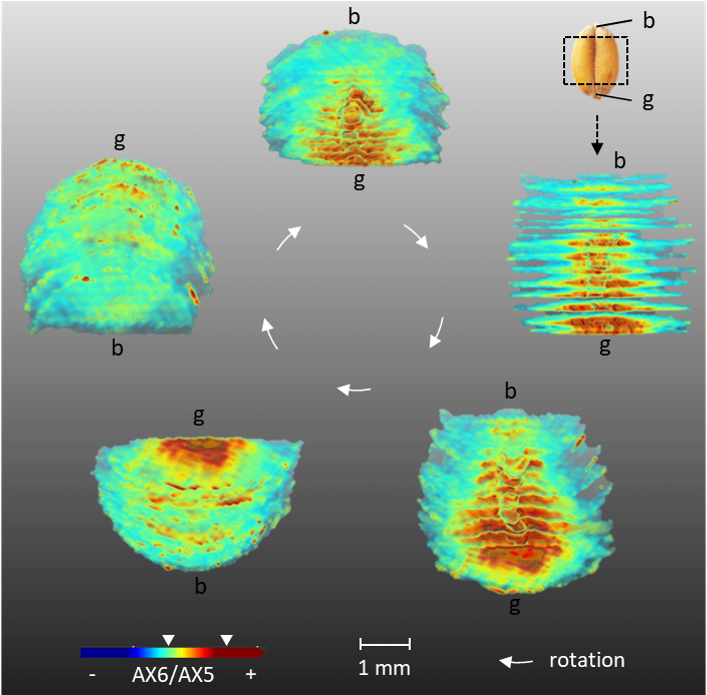
\includegraphics[width=0.6\textwidth]{fig/3Darabinoxylan}
      \label{subfig:3Darabinoxylan}
    \end{subfigure}%
    \begin{subfigure}[t]{0.45\textwidth}
      \centering
      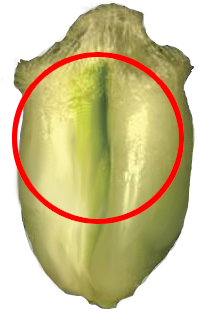
\includegraphics[width=0.35\textwidth]{fig/water_transfer}
      \label{subfig:water_transfer}
    \end{subfigure}%
  \end{figure}

   \underline{Objectif :} identifier de \textbf{nouvelles molécules} dont la distribution spatiale corrèle avec l'eau.\\

\end{frame}

\begin{frame}{Nouvelles données}
  Nouvelles données : \textbf{variété Bobwhite}, 3 stades de
  développement.
  
  \underline{Problèmes :}
  \begin{itemize}
  \item inhomogénéités d'intensité
  \item orientations différentes
  \end{itemize}


   \begin{figure}[ht]
  \centering
  \begin{subfigure}[t]{0.5\textwidth}
    \centering
    \includegraphics<1>[width=0.65\textwidth]{fig/3D_density_aligned_manual0000}%
    \includegraphics<2>[width=0.65\textwidth]{fig/3D_density_aligned_manual0003}%
    \includegraphics<3>[width=0.65\textwidth]{fig/3D_density_aligned_manual0006}%
    \includegraphics<4->[width=0.65\textwidth]{fig/3D_density_aligned_manual0009}
  \end{subfigure}%
    \begin{subfigure}[t]{0.5\textwidth}
    \centering
    \includegraphics<1>[width=0.65\textwidth]{fig/3D_segmentation0000}%
    \includegraphics<2>[width=0.65\textwidth]{fig/3D_segmentation0003}%
    \includegraphics<3>[width=0.65\textwidth]{fig/3D_segmentation0006}%
    \includegraphics<4->[width=0.65\textwidth]{fig/3D_segmentation0009}
  \end{subfigure}%
\end{figure}

\visible<5> {
  $\Rightarrow$ besoin de méthodes \textbf{répétables},
  \textbf{génériques}.
}




    
\end{frame}




\begin{frame}{Chaîne de traitement 3D}


  \begin{enumerate}
  \item<2-> MALDI: \textbf{normalisation} des images
  \item<3-> \textbf{Recalage 3D}
  \item<4-> \textbf{Visualisation} d'images MS en 3D
  \item<5-> Corrélations spatiales avec \textbf{incertitudes}
  \end{enumerate}

  \begin{figure}[ht]
    \centering
    \includegraphics<1>[width=0.76\textwidth]{fig/workflow3D_0}%
    \includegraphics<2>[width=0.76\textwidth]{fig/workflow3D_1}%
    \includegraphics<3>[width=0.76\textwidth]{fig/workflow3D_2}%
    \includegraphics<4>[width=0.76\textwidth]{fig/workflow3D_3}%
    \includegraphics<5>[width=0.76\textwidth]{fig/workflow3D_4}%
  \end{figure}
\end{frame}


\AtBeginSection[]{ \begingroup \setbeamercolor{background
    canvas}{bg=mLightBlue}
  
  \setbeamertemplate{subsection in toc}
  {\leavevmode\leftskip=2em$\bullet$\hskip1em\inserttocsubsection\par}
  \setbeamercolor{section in toc}{fg=paleGrey, bg=mLightBlue}
  \setbeamercolor{local structure}{fg=mLightBlueLighter,bg=mLightBlue}
  \setbeamercolor{section in toc shaded}{fg=mLightBlue, bg=mLightBlue}
  \setbeamertemplate{section in toc}[circle]
  \setbeamertemplate{section in toc shaded}[default][80]
  \setbeamertemplate{section in toc}{\hspace*{1em}\inserttocsection}

  \setbeamercolor{subsection in toc}{fg=paleGrey, bg=mLightBlue}
  \begin{frame}[noframenumbering,plain]
    \frametitle{\textcolor{paleGrey}{Table des matières}}

    \tableofcontents[currentsection, sectionstyle=show/hide,
    hideothersubsections]
  \end{frame}
  \endgroup }


\section{Normalisation d'images de spectrométrie de masse}
\begin{frame}{Normalisation}

  Facteurs de normalisation :
  \begin{enumerate}
  \item Total ion count (TIC) : somme des intensités du spectre
  \item Intensité d'une espèce de référence
  \item Médiane
  \end{enumerate}

  \vspace{0.2cm}

  Généralement, utilisation du \textbf{TIC}: compense les différences
  de mesure entre deux spectres
\end{frame}


\begin{frame}{TIC: problème}
  Variation d'intensité de pics entre deux spectres $\Rightarrow$
  facteurs TIC différents
  
  \begin{figure}[ht]
    \centering
    \includegraphics<1>[width=0.7\textwidth]{fig/normalization1}%
    \includegraphics<2>[width=0.7\textwidth]{fig/normalization2}%
    \includegraphics<3>[width=0.7\textwidth]{fig/normalization3}%
  \end{figure}

\end{frame}

\begin{frame}{TIC: problème}

  \underline{Exemple:} intensité très élevée du pic d'insuline dans le
  pancréas de souris \cite{Deininger_2011}.

  \begin{figure}[ht]
    \centering
    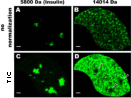
\includegraphics[width=0.7\textwidth]{fig/normalization_defect}
    \caption{}
    \label{fig:normalization_defect}
  \end{figure}

\end{frame}


\begin{frame}{Noise Ion Count}

  \textbf{Idée :} enlever la contribution des pics dans le facteur de
  normalisation.

  \textbf{Calcul :} NIC = TIC - $\sum I_{\text{pics}}$

  \vspace{0.4cm}

  \begin{figure}[ht]
    \centering
    \includegraphics<1>[width=0.7\textwidth]{fig/normalization2}%
    \includegraphics<2>[width=0.7\textwidth]{fig/normalization_sic1}%
    \includegraphics<3>[width=0.7\textwidth]{fig/normalization_sic2}%
    \includegraphics<4>[width=0.7\textwidth]{fig/normalization_sic3}%
    \caption{}
    \label{fig:normalization_sic1}
  \end{figure}


\end{frame}


\section{Recalage 3D}

\begin{frame}{Recalage}

  Méthodes de recalage définies par trois composantes :
  \begin{enumerate}
  \item La \textbf{transformation géométrique} : rigide, affine, non-rigide
  \item La \textbf{métrique} : mesure la similarité entre l'image fixe et mobile, en termes d'intensité ou de géométrie
  \item L'\textbf{optimisation} : méthode pour la détermination du minimum de la métrique \vspace{0.3cm}
  \end{enumerate}
  \vspace{-0.4cm}
  
   \begin{figure}[ht]
    \includegraphics<1>[width=0.6\textwidth]{fig/registration1}%
    \includegraphics<2>[width=0.6\textwidth]{fig/registration2}%
    \includegraphics<3>[width=0.6\textwidth]{fig/registration3}%
    \includegraphics<4>[width=0.6\textwidth]{fig/registration4}%
  \end{figure}

  

\end{frame}



\begin{frame}{Recalage}

  \textbf{Problèmes :} différences d'intensités, orientations très différentes

   \begin{figure}[ht]
    \centering
    \begin{subfigure}[t]{0.5\textwidth}
      \centering
      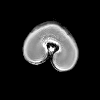
\includegraphics[width=0.65\textwidth]{fig/mri_slice6.png}
    \end{subfigure}%
    \begin{subfigure}[t]{0.5\textwidth}
      \centering
      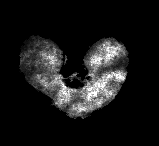
\includegraphics[width=0.65\textwidth]{fig/maldi_slice6}
    \end{subfigure}%

  \end{figure}

  \onslide<2->{
  $\Rightarrow$ Difficile de choisir des \textbf{paramètres appropriés} pour recaler l'ensemble des coupes.
  }
 

\end{frame}

\begin{frame}{Approche pour le recalage}
  
  Approche en deux étapes :
  \begin{enumerate}
  \item recalage affine \textbf{exhaustif} en \textbf{2D}
  \item recalage \textbf{non-rigide} en \textbf{3D}
  \end{enumerate}

  \alert{Recalage exhaustif} : paramètres de transformation \textbf{prédéfinis} $\Rightarrow$ évite de converger vers un \textbf{minimum local}.

  \begin{figure}[ht]
    \centering
    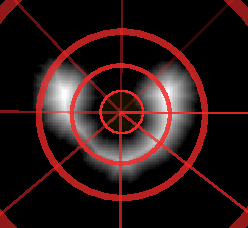
\includegraphics[width=0.4\textwidth]{fig/exhaustive_registration}
    \caption{}
    \label{fig:exhaustive_registration}
  \end{figure}

  
\end{frame}

\begin{frame}{Métrique de similarité}

  Abstraction des intensités : \textbf{transformée en distance}.

  \alert{Transformée en distance} : on associe à chaque pixel sa distance au bord de l'objet.

  \begin{figure}[ht]
    \centering
    \begin{subfigure}[t]{0.5\textwidth}
      \centering
      \includegraphics<1>[width=0.65\textwidth]{fig/mri_slice6.png}%
      \includegraphics<2>[width=0.65\textwidth]{fig/mri_slice6_dt.png}
      \caption{}
      \label{subfig:mri_slice6_dt.png}
    \end{subfigure}%
    \begin{subfigure}[t]{0.5\textwidth}
      \centering
      \includegraphics<1>[width=0.65\textwidth]{fig/maldi_slice6.png}%
      \includegraphics<2>[width=0.65\textwidth]{fig/maldi_slice6_dt.png}
      \caption{}
      \label{subfig:maldi_slice6_dt.png}
    \end{subfigure}%
  \end{figure}

  
\end{frame}

\begin{frame}{Recalage exhaustif}

  Transformation initialisée en alignant les centres de gravité

  \begin{itemize}
  \item La transformation géométrique : espace de paramètres pour rotation et homothétie
  \item La métrique : DT, \textbf{information mutuelle} de Mattes
  \item L'optimisation : \textbf{exhaustive}
  \end{itemize}

  \vspace{-0.2cm}
  \begin{figure}[ht]
    \centering
    \includegraphics<1>[width=0.65\textwidth]{fig/metric_exh_0}%
    \includegraphics<2>[width=0.65\textwidth]{fig/metric_exh_1}%
    \includegraphics<3>[width=0.65\textwidth]{fig/metric_exh_2}
    \label{fig:metric_2}
  \end{figure}

\end{frame}

\begin{frame}{Recalage non-rigide}
  Déformations $\Rightarrow$ valeurs de transformée en distance

  \vspace{0.4cm}
  
  \textbf{Nouvelle métrique}: somme des moindres carrés avec mise
  à jour de la transformée en distance.

  \begin{figure}[ht]
  \centering
  \begin{subfigure}[t]{0.2\textwidth}
    \centering
    
\includegraphics[width=0.95\textwidth]{fig/registration_reference}
    \caption{}
    \label{subfig:registration_reference}
  \end{subfigure}%
  \begin{subfigure}[t]{0.2\textwidth}
    \centering
    
\includegraphics[width=0.95\textwidth]{fig/registration_target}
    \caption{}
    \label{subfig:registration_target}
  \end{subfigure}%
  \begin{subfigure}[t]{0.2\textwidth}
    \centering
    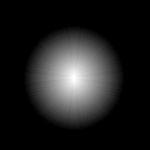
\includegraphics[width=0.95\textwidth]{fig/registration_reference_dt}
    \caption{}
    \label{subfig:registration_dt_reference}
  \end{subfigure}%
  \begin{subfigure}[t]{0.2\textwidth}
    \centering
    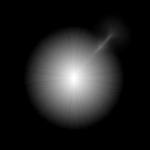
\includegraphics[width=0.95\textwidth]{fig/registration_target_dt_interpol.png}
    \caption{}
    \label{subfig:registration_dt_target_interpol}
  \end{subfigure}%
  \begin{subfigure}[t]{0.2\textwidth}
    \centering
    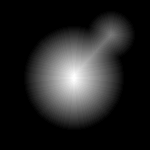
\includegraphics[width=0.95\textwidth]{fig/registration_target_dt}
    \caption{}
    \label{subfig:registration_dt_target}
  \end{subfigure}%
\end{figure}
\end{frame}


\begin{frame}{Recalage non-rigide}
  
  \begin{columns}
    \begin{column}[t]{0.6\textwidth}
      \textbf{Méthodes variationnelles} : modélisation d'une force d'attraction des pixels, sous la forme d'un \textbf{champ de vecteurs}. \vspace{0.2cm}

      \begin{enumerate}
      \item Forces externes : métrique $\textcolor{red}{\mathcal{D}}$ : somme moindres carrés avec MÀJ
      \item Forces internes : terme de \textbf{régularisation} $\textcolor{blue}{\mathcal{S}}$
      \end{enumerate}

      \[
        \mathcal{J}[y] = \textcolor{red}{\mathcal{D}[\mathcal{T}[y], \mathcal{R}]} + \textcolor{blue}{\mathcal{S}[y]} \xrightarrow{y} \min
      \]
      
      % \[
      %   \mathcal{J}[y] = \textcolor{red}{\mathcal{D}[\mathcal{T}[y], \mathcal{R}]} + \textcolor{blue}{\mathcal{S}[y]} \xrightarrow{y} \min
      % \]
    \end{column}
    \begin{column}[t]{0.4\textwidth}
      \begin{figure}[ht]
        \centering
        \includegraphics<1>[width=0.95\textwidth]{fig/registration_nonrigid_vectorfield_2}%
        \includegraphics<2>[width=0.95\textwidth]{fig/registration_nonrigid_vectorfield_10}%
        \includegraphics<3>[width=0.95\textwidth]{fig/registration_nonrigid_vectorfield_30}%
        \includegraphics<4>[width=0.95\textwidth]{fig/registration_nonrigid_vectorfield}%
      \end{figure}
    \end{column}
  \end{columns}
\end{frame}




\begin{frame}{Analyse statistique}
  
  \begin{columns}
    \begin{column}[t]{0.6\textwidth}
      \begin{enumerate}
      \item Réduction de la dimension des images 2D par \textbf{NMF} 
      \item \textbf{Projection} de l'image IRM sur les axes de la NMF
      \item Sélection des images MALDI \textbf{les plus proches} de la projection
        de l'image IRM 
      \end{enumerate}
    \end{column}
    \begin{column}[t]{0.4\textwidth}
      \begin{figure}[ht]
        \centering
        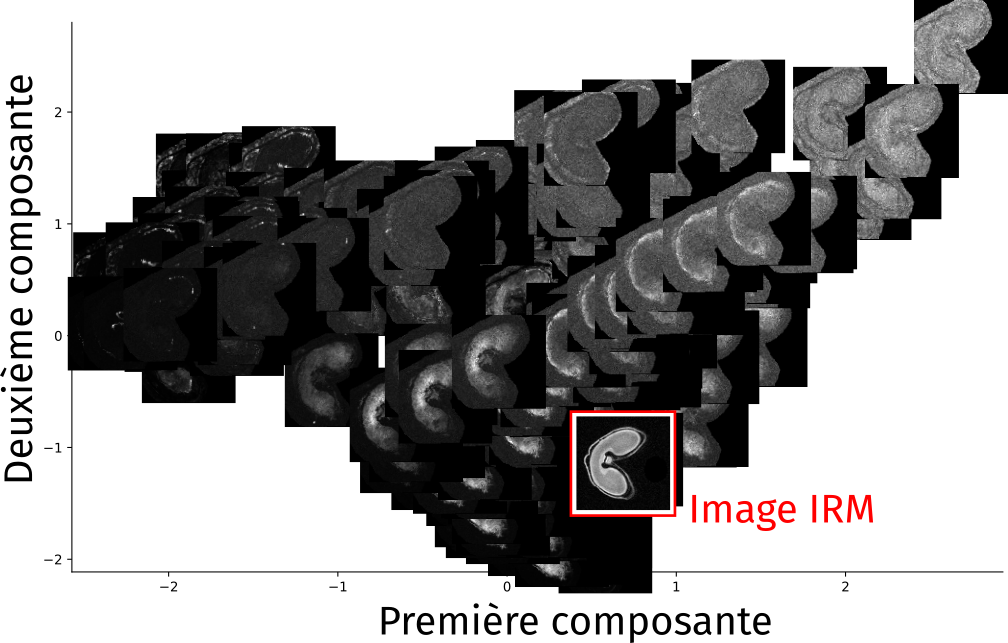
\includegraphics[width=0.95\textwidth]{fig/pca_big3}
      \end{figure}
    \end{column}
  \end{columns}
\end{frame}

\begin{frame}{Analyse statistique}
  Identification des \textbf{molécules en MALDI corrélant avec les images IRM}.

  \textbf{Problème :} les régions apparentes dans les deux modalités ne sont pas nécessairement alignées.

  \begin{figure}[ht]
  \centering
  \begin{subfigure}[t]{0.33\textwidth}
    \centering
    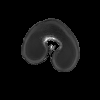
\includegraphics[width=0.9\textwidth]{fig/t2_6_original}
    \caption{}
    \label{subfig:t2_6_original}
  \end{subfigure}%
  \begin{subfigure}[t]{0.33\textwidth}
    \centering
    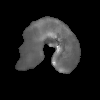
\includegraphics[width=0.9\textwidth]{fig/msi_6_original}
    \caption{}
    \label{subfig:msi_6_original}
  \end{subfigure}%
  \begin{subfigure}[t]{0.33\textwidth}
    \centering
    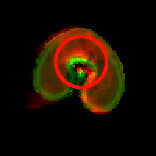
\includegraphics[width=0.9\textwidth]{fig/overlay_t2_6_original}
    \caption{}
    \label{subfig:overlay_t2_6_original}
  \end{subfigure}%
\end{figure}

\end{frame}


\begin{frame}{Analyse statistique}
  \textbf{Contribution :} Recalage exhaustif impliquant des translations des images de composantes


  \begin{figure}[ht]
    \centering
    \includegraphics<1>[width=0.9\textwidth]{fig/translation_nmf_0}%
    \includegraphics<2>[width=0.9\textwidth]{fig/translation_nmf_1}%
    \includegraphics<3>[width=0.9\textwidth]{fig/translation_nmf_2}%
    \includegraphics<4>[width=0.9\textwidth]{fig/translation_nmf_3}%
  \end{figure}

  
\end{frame}







\section{Visualisation}


\begin{frame}{Visualisation 3D}
  Outil pour la visualisation de fichiers imzML 3D:
  \begin{itemize}
  \item Python3
  \item Bibliothèques \texttt{vedo}, \texttt{vtk} et \texttt{pyqt5}
  \end{itemize}

  \vspace{-0.2cm}
  
  \begin{figure}[ht]
    \centering
    \includegraphics<1>[width=0.95\textwidth]{fig/visu}%
    \includegraphics<2>[width=0.95\textwidth]{fig/visu2}%
    \includegraphics<3>[width=0.95\textwidth]{fig/visu3}
    \caption{}
    \label{fig:visu}
  \end{figure}

\end{frame}

\begin{frame}{Visualisation 3D}
  
  Rendu volumique :
  \begin{figure}[ht]
    \centering
    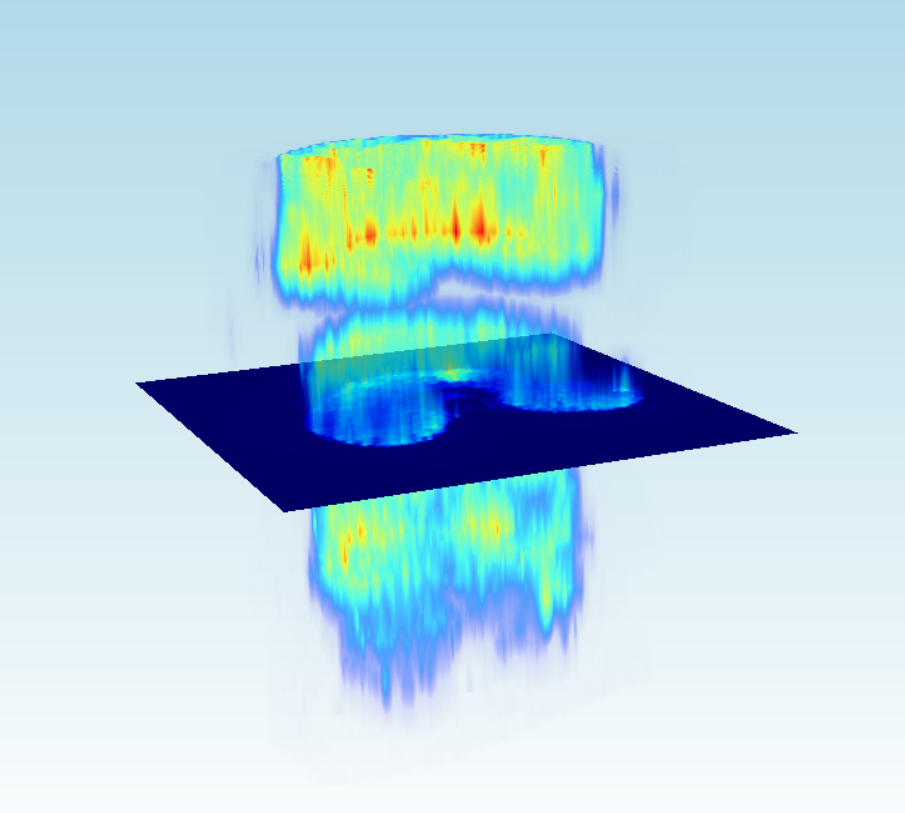
\includegraphics[width=0.5\textwidth]{fig/visu_3d.png}
    \caption{}
    \label{fig:visu_3d.png}
  \end{figure}

\end{frame}

\section{Résultats}
\begin{frame}{Normalisation}

  Compensation de certains artefacts de normalisation:
  
  \begin{figure}[ht]
    \centering
    \begin{subfigure}[t]{0.3\textwidth}
      \centering 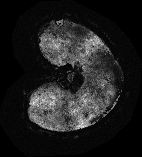
\includegraphics[width=0.9\textwidth]{fig/real_tic}
      \caption{TIC}
      \label{subfig:real_tic}
    \end{subfigure}%
    \begin{subfigure}[t]{0.3\textwidth}
      \centering 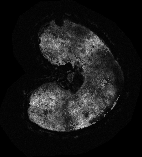
\includegraphics[width=0.9\textwidth]{fig/real_sic}
      \caption{NIC}
      \label{subfig:real_sic}
    \end{subfigure}%
    \begin{subfigure}[t]{0.35\textwidth}
      \centering 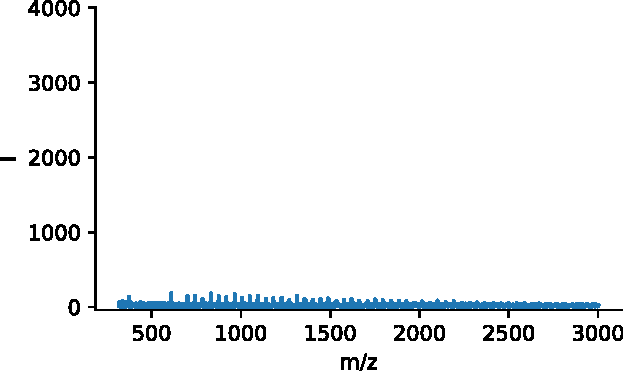
\includegraphics[width=0.9\textwidth]{fig/real_defect}
      \caption{}
      \label{subfig:real_defect}
    \end{subfigure}%
  \end{figure}
\end{frame}

\begin{frame}{Recalage}

  \vspace{-0.3cm}
  Proportion de pixels en commun:
  \begin{itemize}
  \item \textbf{simple} sans transformée en distance: \textbf{77.9\%}
  \item \textbf{(b)} \textbf{exhaustif} avec transformée en distance: \textbf{84.6\%}
  \item \textbf{(c)} \textbf{variationnel} sans mise à jour de la DT : \textbf{90.2\%}
  \item \textbf{(d)} \textbf{variationnel} avec mise à jour de la DT : \textbf{93.2\%}
  \end{itemize}

  \begin{figure}[ht]
  \centering
  \begin{subfigure}[t]{0.25\textwidth}
    \centering
    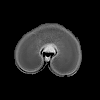
\includegraphics[width=0.95\textwidth]{fig/registration_wheat_mri}
    \caption{}
    \label{subfig:registration_wheat_mri}
  \end{subfigure}%
  \begin{subfigure}[t]{0.25\textwidth}
    \centering
    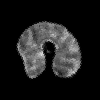
\includegraphics[width=0.95\textwidth]{fig/registration_wheat_affine}
    \caption{}
    \label{subfig:registration_wheat_affine}
  \end{subfigure}%
  \begin{subfigure}[t]{0.25\textwidth}
    \centering
    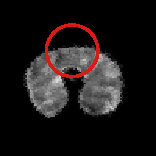
\includegraphics[width=0.95\textwidth]{fig/registration_wheat_ssd}
    \caption{}
    \label{subfig:registration_wheat_ssd}
  \end{subfigure}%
  \begin{subfigure}[t]{0.25\textwidth}
    \centering
    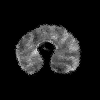
\includegraphics[width=0.95\textwidth]{fig/registration_wheat_dtssd}
    \caption{}
    \label{subfig:registration_wheat_dtssd}
  \end{subfigure}%
\end{figure}
\end{frame}

\begin{frame}{Analyse statistique}
  Meilleure fidélité à l'image IRM originale avec \textbf{(b)}
  \textbf{translation} des composantes, plutôt que \textbf{(c) sans}.
    \begin{figure}[ht]
  \centering
  \begin{subfigure}[t]{0.3\textwidth}
    \centering
    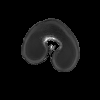
\includegraphics[width=0.95\textwidth]{fig/t2_6_original}
    \caption{}
    \label{subfig:t2_6_original}
  \end{subfigure}%
  \begin{subfigure}[t]{0.3\textwidth}
    \centering
    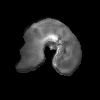
\includegraphics[width=0.95\textwidth]{fig/reconstruction_t2_translated.png}
    \caption{}
    \label{subfig:reconstruction_t2_translated.png}
  \end{subfigure}%
    \begin{subfigure}[t]{0.3\textwidth}
    \centering
    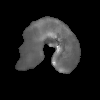
\includegraphics[width=0.95\textwidth]{fig/msi_6_original.png}
    \caption{}
    \label{subfig:reconstruction_t2_translated.png}
  \end{subfigure}%
\end{figure}

\end{frame}

\begin{frame}{Mise en corrélation}

  Résultats sur la \textbf{variété Bobwhite} (stade 250 DJ):

    \begin{figure}[ht]
    \centering
    \begin{subfigure}[t]{0.33\textwidth}
      \centering
      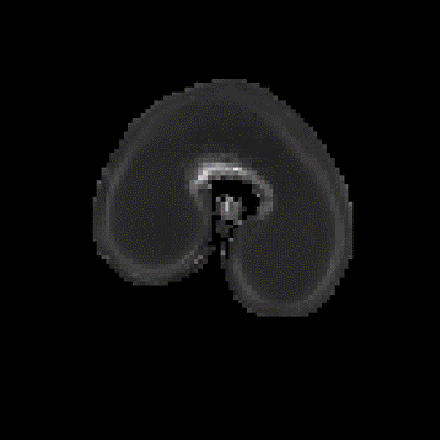
\includegraphics[width=0.9\textwidth]{fig/mri_slice8_250}
      \caption{IRM $T_2^*$}
      \label{subfig:mri_slice8_250}
    \end{subfigure}%
    \begin{subfigure}[t]{0.33\textwidth}
      \centering
      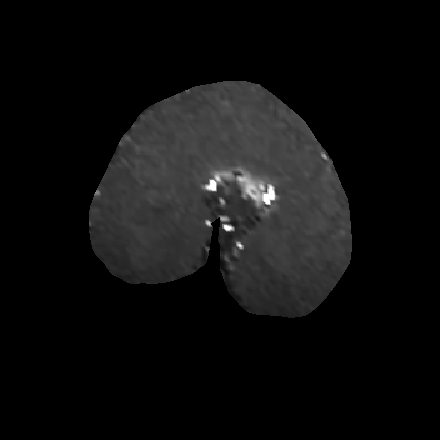
\includegraphics[width=0.9\textwidth]{fig/zonetir_2}
      \caption{$\dfrac{\text{AX6}}{\text{AX5}}$}
      \label{subfig:zonetir_0}
    \end{subfigure}%
    \begin{subfigure}[t]{0.33\textwidth}
      \centering
      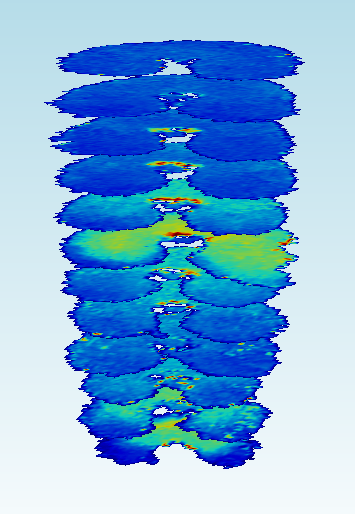
\includegraphics[width=0.7\textwidth]{fig/3D_250DJ}
      \caption{$\dfrac{\text{AX6}}{\text{AX5}}$ (en 3D)}
      \label{subfig:3D_250DJ}
    \end{subfigure}%

  \end{figure}

   $\Rightarrow$ Rapport $\dfrac{\text{AX6}}{\text{AX5}}$ : lien entre \textbf{degré de substitution} des AX et \textbf{mobilité de l'eau} \cite{Fanuel18}.

\end{frame}



\section{Bilan}

\begin{frame}{Bilan}

  Chaîne de traitement \textbf{ajustée} pour le \textbf{traitement
    automatique} d'images 3D.

  Résultats au stade 250 DJ: confirment les \textbf{résultats
    précédents}.

  \vspace{0.4cm}

  Perspectives:
  \begin{itemize}
  \item Recalage avec des \textbf{variations locales d'échelle}.
  \item Analyse statistique \textbf{complète en 3D}.
  \end{itemize}


\end{frame}

\begin{frame}{Variations locales d'échelle}

  La transformation en distance est sensible aux variations d'échelle.

  \visible<3->{
    \textbf{Idée : } normaliser les valeurs de transformée en distance
    par les valeurs d'\textbf{échelle locale} (rayon de l'objet).
  }
  

  \begin{figure}[ht]
    \flushleft
    \begin{subfigure}[t]{0.2\textwidth}
      \centering
      
\includegraphics[width=0.95\textwidth]{fig/prospect_reference}
      \caption{}
      \label{subfig:prospect_reference}
    \end{subfigure}%
    \begin{subfigure}[t]{0.2\textwidth}
      \centering
      
\includegraphics[width=0.95\textwidth]{fig/prospect_target}
      \caption{}
      \label{subfig:prospect_target}
    \end{subfigure}%
    \only<2->{%
    \begin{subfigure}[t]{0.2\textwidth}
      \centering
      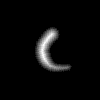
\includegraphics[width=0.95\textwidth]{fig/prospect_registered_target}
      \caption{}
      \label{subfig:prospect_registered_target}
    \end{subfigure}%
    }%
    \only<3->{%
      \begin{subfigure}[t]{0.2\textwidth}
        \centering
        
\includegraphics[width=0.95\textwidth]{fig/prospect_normalized_dt}
        \caption{}
        \label{subfig:prospect_normalized_dt}
      \end{subfigure}%
    }%
    \only<4->{%
      \begin{subfigure}[t]{0.2\textwidth}
        \centering
        
\includegraphics[width=0.95\textwidth]{fig/prospect_registered_target_normalized}
        \caption{}
        \label{subfig:prospect_registered_target_normalized}
      \end{subfigure}%
    }
  \end{figure}

\end{frame}






\appendix
\setbeamertemplate{headline}{%
  % \nointerlineskip
  % \begin{beamercolorbox}[wd=\paperwidth,leftskip=0.5cm,ht=0pt,dp=0pt]{block title}%
  %   \usebeamerfont{page number in head/foot}{\insertsection}
  % \end{beamercolorbox}%
  % \if@useTitleProgressBar
  % \nointerlineskip
  % % \vspace{-0.7cm}
  % \begin{beamercolorbox}[wd=\paperwidth,ht=0pt,dp=5pt]{section}
  %   \progressbar@titleprogressbar
  % \end{beamercolorbox}
  % \fi
  % \nointerlineskip
}

% \setbeamertemplate{frametitle}{%
%   \begin{beamercolorbox}[wd=\paperwidth,leftskip=0.7cm,rightskip=0.3cm,ht=0pt,dp=0pt]{frametitle}
%     \usebeamerfont{frametitle}\MakeLowercase{\protect\insertframetitle}
%   \end{beamercolorbox}
% }

\begin{frame}[allowframebreaks]
  \frametitle{Références}
  \setbeamertemplate{bibliography item}{$\bullet$}
  \bibliographystyle{apalike}
  \scriptsize{
    \bibliography{main}
  }
\end{frame}



\end{document}
